While lost on the long walk from the college to the UQ Centre, you have stumbled across the entrance to a secret cave system running deep under the university. The entrance is blocked by a security system consisting of $N$ consecutive doors, each door behind the previous; and N switches, with each switch connected to a different door.

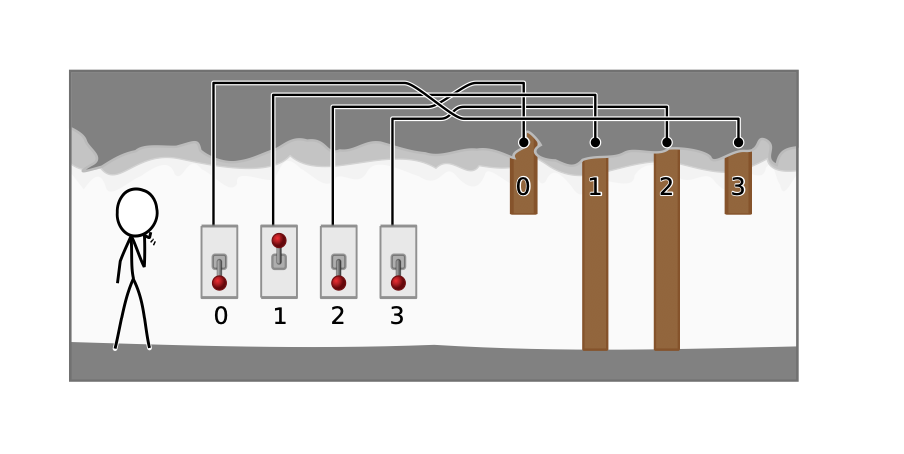
\includegraphics{cave1.png}

The doors are numbered $0, 1, \dots, N - 1$ in order, with door $0$ being closest to you. The switches are also numbered $0, 1, \dots, N - 1$, though you do not know which switch is connected to which door.

The switches are all located at the entrance to the cave. Each switch can either be in an \textit{up} or \textit{down} position. Only one of these positions is correct for each switch. If a switch is in the correct position then the door it is connected to will be open, and if the switch is in the incorrect position then the door it is connected to will be closed. The correct position may be different for different switches, and you do not know which positions are the correct ones.

You would like to understand this security system. To do this, you can set the switches to any combination, and then walk into the cave to see which is the first closed door. Doors are not transparent: once you encounter the first closed door, you cannot see any of the doors behind it.

You have time to try $70\,000$ combinations of switches, but no more. Your task is to determine the correct position for each switch, and also which door each switch is connected to.

You should submit a file that implements the procedure \t{exploreCave()}. This may call the grader function \t{tryCombination()} up to $70\,000$ times, and must finish by calling the grader procedure \t{answer()}. These functions and procedures are described below.

Grader Function \t{tryCombination()}:

\t{int tryCombination(int S[]);}

The grader will provide this function. It allows you to try a combination of switches, and then enter the cave to determine the first closed door. If all doors are open, the function will return $-­1$. This function runs in $O(N)$ time; that is, the running time is at worst proportional to $N$.

This function may be called at most $70\,000$ times. 

Parameters:
\begin{itemize}
\item $S$: An array of length $N$, indicating the position of each switch. The element $S[i]$ corresponds to switch $i$. A value of $0$ indicates that the switch is up, and a value of $1$ indicates that the switch is down.
\item \textit{Returns}: The number of the first door that is closed, or ­$-1$ if all doors are open.
\end{itemize}


       
Grader Procedure \t{answer()}:

\t{void answer(int S[], int D[]);}

Call this procedure when you have identified the combination of switches to open all doors, and the door to which each switch is connected.

Parameters:
\begin{itemize}
\item $S$: An array of length $N$, indicating the correct position of each switch. The format matches that of the function \t{tryCombination()} described above.
\item $D$: An array of length $N$, indicating the door each switch is connected to. Specifically, element $D[i]$ should contain the door number that switch $i$ is connected to.
\item \textit{Returns}: This procedure does not return, but will cause the program to exit.
\end{itemize}

Your Procedure \t{exploreCave()}:

\t{void exploreCave(int N);}

Your submission must implement this procedure.

This function should use the grader routine \t{tryCombination()} to determine the correct position for each switch and the door each switch is connected to, and must call \t{answer()} once it has determined this information.

Parameters:
\begin{itemize}
\item $N$: The number of switches and doors in the cave.
\end{itemize}
